% TODO: explain that tropes are not covered academically, I am attempting to
% make tropes academically respectable
% TODO: make it clear at the start that we are choosing these examples as a way
% to demonstrate tropes ability to create abstractions
% TODO: parental abandonment might need extra characters
% TODO: connect character role (such as Comedic Sociopath) to our emotional model
% TODO: connect our idea of phases with landmarks in plans / knowledge
% representation literature
% do also need to demonstrate adequate knowledge of planners
% TODO: put TropICAL / instal fragments in column in appendix, pull out relevant
% features to describe in the chapter
\chapter{Tropes as Story Components}
\label{cha:tropes}
This chapter describes the foundations of our new formalism for narrative: story
tropes. Though our use of tropes for the description of stories has many
advantages, the main advantage that we will focus on throughout this thesis is
that they provide a means of creating new abstractions from existing tropes. For
more detail on how tropes allow us to do this, please see section~\ref{sec:abstractable}

Though story tropes may be a familiar concept to many outside of the academic
community, they do not appear in the literature in either fields Computer Science or
Narratology at the time of writing. Therefore this chapter contains a thorough
description of what a story trope is, along with several examples.

As previously described in chapter~\ref{cha:introduction}, tropes are
patterns that appear throughout various different media. Once one is familiar
with a trope, it becomes easy to identify its use in any story. Take, for
example, the \emph{Hero's Journey} trope first described in
chapter~\ref{cha:introduction}. It is a template which is repeated so often in
many different media, stories and contexts that it is instantly recognised even
by those that are completely unfamiliar with the concept of tropes.

% Bit about difference between tropes and cliches

In this section we examine the concept of a ``trope'', deconstructing examples
to demonstrate widely-recognised trope patterns, and exploring tropes that
operate at different levels of abstraction within a story. At the end of the
section we identify a formal definition of a trope, and how it fits within the
wider context of a story.

% TODO NUMBER
% TODO list of examples where tropes appear from jurisin paper
% TODO TVtropes screenshot figure
% TODO describe the periodic trope groups
\section{Tropes: a ``Folksonomy'' of Story Components}
The existence of a website called ``TV Tropes''~\citep{tvtropes} makes the discovery of example
tropes very simple. TV Tropes is a wiki for tropes, containing over 27,000
trope descriptions, along with the media that they appear in. For example, the
``The Empire'' trope appears in \emph{Star Wars}, Asimov's \emph{Foundation}
trilogy, the \emph{Hunger Games} books and films, and the \emph{Final Fantasy}
series of games, and a great many more stories in media.


\begin{figure}[!t]
\centerline{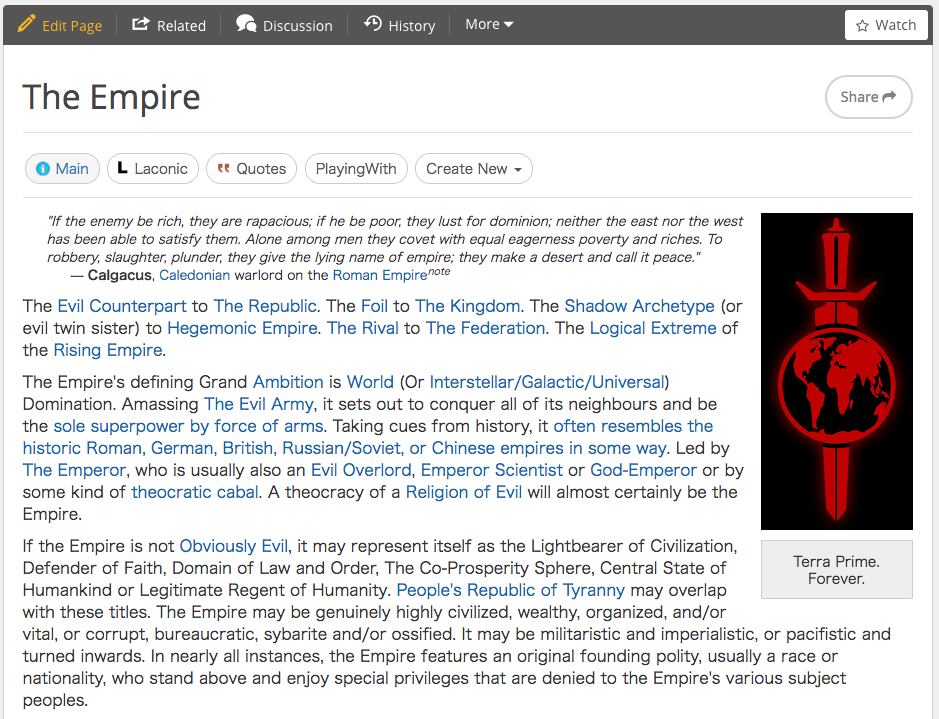
\includegraphics[height=5in]{evilEmpire.png}}
\caption{A screenshot of the ``The Empire'' wiki page from TV Tropes} \label{fig:evil-empire}
\end{figure}

Figure~\ref{fig:evil-empire} shows a screenshot of the ``The Empire'' page on the
website. It clearly shows the description of the trope at the top of the page,
and there are also instances of its use across different media at the bottom.

Tropes can also describe character archetypes. For example, this is how TV
Tropes describes \emph{Anti-Hero} characters:

\begin{quote}
An Archetypal Character who is almost as common in modern fiction as the Ideal Hero, an antihero is a protagonist who has the opposite of most of the traditional attributes of a hero. They may be bewildered, ineffectual, deluded, or merely apathetic. More often an antihero is just an amoral misfit. While heroes are typically conventional, anti-heroes, depending on the circumstances, may be preconventional (in a "good" society), postconventional (if the government is "evil") or even unconventional. Not to be confused with the Villain or the Big Bad, who is the opponent of Heroes (and Anti-Heroes, for that matter).
  \end{quote}

TV Tropes further clarifies that there are even further subdivisions of
Anti-Hero, depending on just how evil or cynical the character is. Batman, for
example, would be a highly cynical Anti-Hero who is nevertheless morally good.

Shakespeare's Macbeth is a character who becomes more and more of an evil Anti-Hero, until he is too morally evil
to still be a Hero and instead becomes a Tragic Villain.

Tropes can be very specific, referring to individual lines of dialogue.
One example is ``We Will Meet Again'':

\begin{quote}
The standard phrase when the villain finds that he has been defeated by the heroes and there is no point in staying around with the immediate Evil Plan foiled.
\end{quote}

Tropes can also be very abstract, referring to particular genres, types of
story, or events in a story that move the action forward. Other than the
previously mentioned ``Hero's Journey'' and ``The Empire'' tropes, another
example could be the ``Hilarity Ensues'' trope:

\begin{quote}
Actions that are dangerous or illegal often lead to injury, arrest, job dismissal, expulsion from school, deportation, or other dire consequences. Thankfully for our fictional friends, both the Rule of Cool and the Rule of Funny keep them safe (the latter more prominently).
\end{quote}

\emph{Metatropes} are tropes about tropes, often intended as a knowing wink to
the trope-savvy audience. One such example is ``Lampshade Hanging'', which TV
Tropes describes as:

\begin{quote}
...the writers' trick of dealing with any element of the story that threatens the audience's Willing Suspension of Disbelief, whether a very implausible plot development, or a particularly blatant use of a trope, by calling attention to it and simply moving on.
\end{quote}

In fact, even if an audience is unaware of the concept of tropes, they may be aware
of the recurring patterns and themes that they describe. This enables
genre-savvy (and especially postmodern) writers to play with the audience's
expectations. Ways to do this with tropes could include \emph{inversion}
(reversing the trope),
\emph{subversion} (making it look like the trope will happen, but then not using
it after all), \emph{parody} (using the trope in an over-the-top, exaggerated
manner) and \emph{deconstruction} (using the trope in a straightforward manner,
but in way which forces the audience to analyse the trope itself).

Take, for example, the well-known ``The Butler Did It'' trope from murder
mystery stories, where the butler of the house is revealed to be the murderer at
the end of the story. TV Trope describes ways that an author could ``play'' with this trope:

\begin{compactitem}
  \item \textbf{Subvert} it: The butler is the prime suspect at the beginning, and is later found innocent.
  \item \textbf{Invert} it: The butler is the victim. Or the butler solved the crime. Or every suspect except the butler was part of the crime.
  \item \textbf{Parody} it: Butlers could learn their trade at butler college where they are taught cleaning, cooking, and murdering.
  \item \textbf{Deconstruct} it: The butler is a revolutionary serial killer, who purposely takes jobs as butlers to murder his rich masters. All the unfortunate implications of class warfare that this suggests are brought up and discussed.
\end{compactitem}

Many other examples of using tropes in this way can be found on the ``Playing
with a Trope'' page of the TV Tropes website~\cite{playing-tropes}.


\begin{figure}[!t]
\centerline{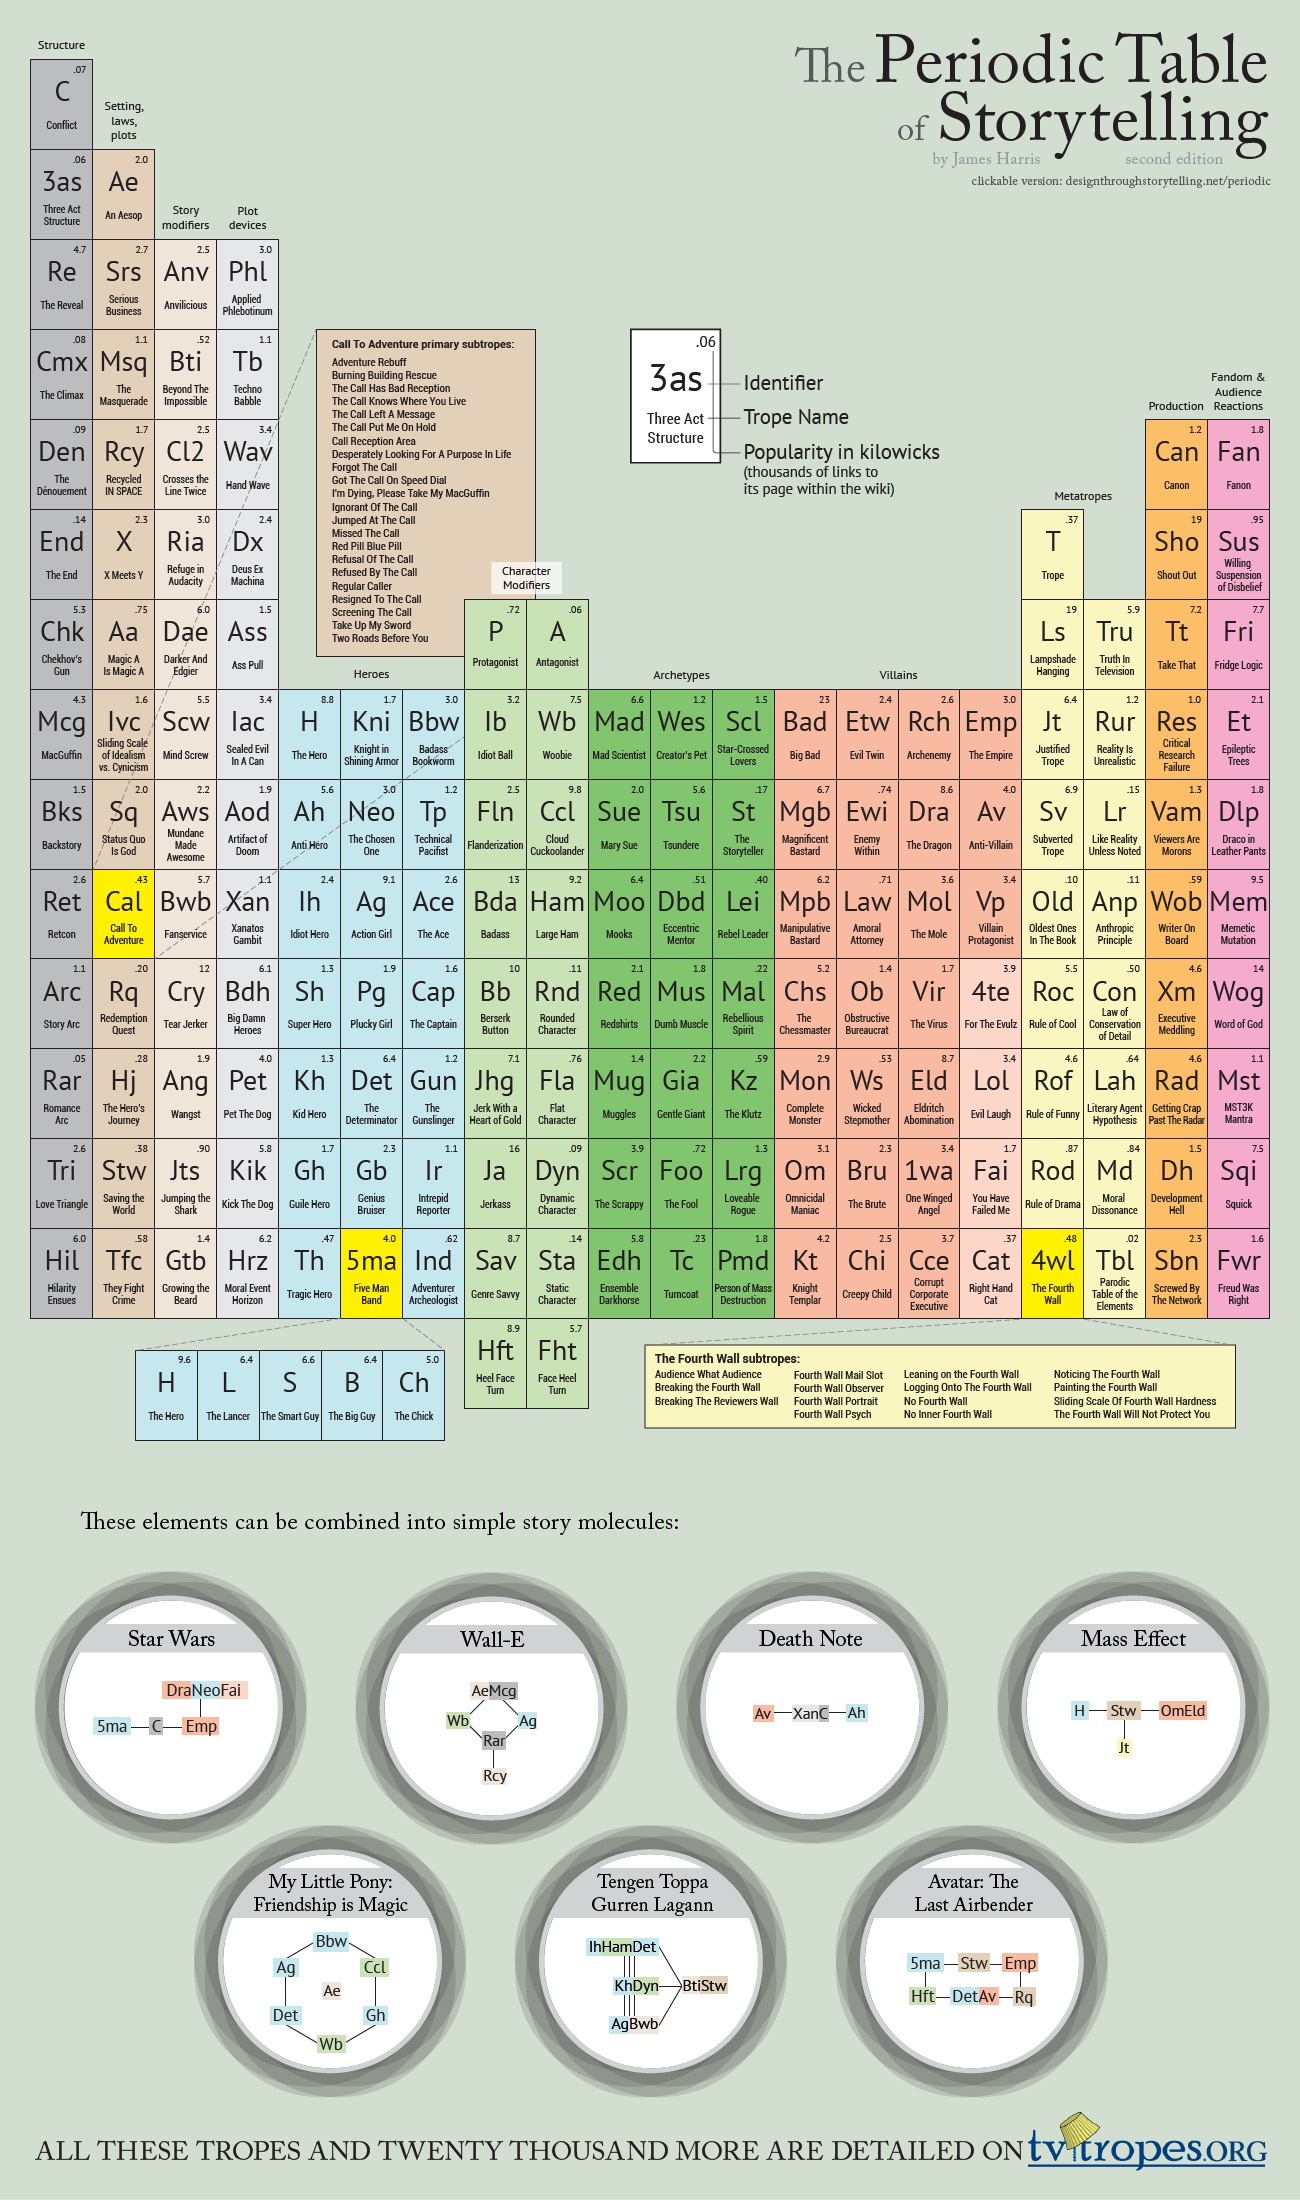
\includegraphics[height=9in]{periodicTable.png}}
\caption{The ``Periodic Table of Storytelling'', original by James Harris
  (http://jamesharris.design/periodic/), poster format by Deviant Art user Dawn
  Paladin (http://dawnpaladin.deviantart.com/art/The-Periodic-Table-of-Storytelling-Second-Edition-425816342)} \label{fig:periodic-table}
\end{figure}

A large and highly active community of users and contributors exists around TV
Tropes. In addition to creating content for and curating the content on the
website, they also work to create useful ways to visualise the usage of tropes
in stories. For example, The Periodic Table of
Storytelling~\citep{periodicTableOfStorytelling} is a visualisation of tropes as
``elements'' in the ``molecules'' of a story. The table itself
(fig.~\ref{fig:periodic-table}) arranges the tropes into different ``groups''
according to the part of a story that they operate on. The leftmost groups
describe the story as a whole, describing its \emph{structure} (``Three Act
Structure'', ``MacGuffin'', ``Chekov's Gun''), \emph{story
  modifiers} (``Darker and Edgier'', ``Tear Jerker'', ``Jumping the Shark''),
and \emph{plot devices} (``Hand Wave'', ``Techno Babble'', ``Xanatos Gambit'').
In the centre of the table are different types of character such as
\emph{Heroes} (``Anti Hero'', ``Action Girl'', ``The Gunslinger''),
\emph{Archetypes} (``Mad Scientist'', ``The Fool'', ``Loveable Rogue'') and
\emph{Villains} (``Evil Twin'', ``The Empire'', ``Obstructive Bureaucrat''). The
right third of the table contains self-referential tropes such as
\emph{metatropes} (``Lampshade Hanging'', ``Subverted Trope'', ``The Fourth
wall''), and \emph{fandom and audience reactions} (``Fanon'', ``Fridge Logic'',
``Freud Was Right'').

The story is then visualised as a molecule composed from tropes, linked together as
atoms (shown at the bottom of fig.~\ref{fig:periodic-table}).

This visualisation demonstrates the core idea of our use of tropes as reusable
story components, but the ``molecule'' metaphor is unsuitable for a couple of
reasons. Firstly, linking tropes together as atoms in a molecule does not
communicate the different levels of abstraction at which tropes operate.
Considering that our main purpose for choosing tropes as our method of
describing narrative components, this means that the ``molecule'' metaphor used
by the author does not match our intentions. The
``Hero's Journey'' trope, for example, would describe the narrative arc as a
whole, while the ``Comeuppance'' trope would describe just a single scene in the
story. The metaphor is also not ideal because it presents orthogonal concepts
together in a story with no indication of which part of a narrative they affect.
A ``scoundrel sidekick'' could be linked together with a ``breaking the fourth
wall'' trope, even though one trope relates to a certain character, and the
other may describe a single line of dialogue or action that occurs at a specific
point in the story. 

Also, the arrangement and linking of the tropes in the example molecules is
quite arbitrary. The examples given on the \emph{periodic table} web site form
interesting shapes, but do not follow a consistent logic. In the \emph{Star
  Wars} molecule, for example, the ``Five Man Band'', ``Conflict'' and ``The
Empire'' tropes are linked in a straight line suggesting a linear sequence, but
three further tropes (``The Dragon'', ``The Chosen One'' and ``You Have Failed
Me'') are all linked to the ``The Empire'' trope in the molecule. While ``The
Dragon'' refers to the Death Star in the movie, the ``The Chosen One'' trope is
more closely linked to Luke Skywalker's Hero role. The ``You Have Failed Me''
trope refers to a specific scene where villain Darth Vader punishes an
under performing henchman with choking. It is not clear why the creator decided
to link these specific tropes to the ``The Empire''
trope.

Similarly, in the \emph{GhostBusters} example, the ``Five Man Band'' and ``Mad
Scientist'' tropes appear together in the same ``atom'', which are linked to
``Sealed Evil in a Can'' and ``Hilarity Ensues''. Again, it is not clear why
those particular tropes are arranged together into the same atoms, or why they
are linked together in this way. The most likely explanation is that this
visualisation of the way that tropes link together in a story is not intended as
a serious way to formalise stories, and is merely a ``fun'' example.

Taking this visualisation as inspiration, we develop our concept of tropes as
logical, reusable components for the formal description of stories. Importantly,
we develop a way to nest tropes within other tropes as subtropes as a way to
describe tropes acting at different levels of abstraction.

% TODO rip the whole bit from the lit review? Consider it at least
\section{Why Use Tropes?}
% Write about ability to abstract, give story examples vs Propp
% This is pretty much covered in the lit review

Returning to the shortcomings of existing narrative formalisms we describe in
section~\ref{litrev-discussion}, we now describe how tropes are suitable for use
as a narrative formalism that is able to overcome these limitations.

\subsection{A Means of Abstraction}
\label{sec:abstraction}
Most tropes exist in a hierarchy of tropes, with parent tropes such as the
\emph{Quest} containing child tropes such as \emph{Redemption Quest},
\emph{Sidequest} or a \emph{Quest for Identity}. These child-tropes inherit some
of the characteristics of their parents, but add subtle or major changes. For
example, a \emph{Quest for Identity} follows the \emph{Quest} format, but is
constrained so that the item the hero is questing after is the hero's own
identity. This is a mechanism of \emph{inheritance}, so one can imagine using
such a process to avoid duplication of effort when authoring new tropes by only
expressing how a trope differs from its parent.

\begin{figure}[!t]
\centerline{
\includegraphics[height=1.5in]{freytag.png}}
\caption{Freytag's Pyramid} \label{fig:freytag}
\end{figure}

Another method of abstraction is to express tropes that are contained as parts
of larger tropes. The example we described in section~\ref{litrev-discussion}
describes how the ``Quest'' trope could form just one part of a larger trope
such as the ``Hero's Journey''. Another example of this would be the
\textbf{Three Act Structure} (also known as Freytag's Pyramid) shown in fig.~\ref{fig:freytag}, which describes the shape of a
story in terms of rising and falling levels of drama. This could be split into
five (or perhaps more) sub-tropes:

\begin{compactitem}
  \item \textbf{Exposition}: The setting of the scene, providing any background
    information that is relevant to the story.
  \item \textbf{Rising Action}: A series of event drive the story forward, each
    increasing in dramatic intensity.
  \item \textbf{Climax}: The turning point of the story. Some fateful event
    occurs as a result of the rising action, which could be a battle between the
    hero and the villain, for example.
  \item \textbf{Falling Action}: The consequences of the climax play out, and
    the story shows how the characters are affected.
  \item \textbf{Denouement}: This is the final resolution, where all the ``loose
    ends'' of the story are tied up.
\end{compactitem}

This means that if we already have trope definitions for the ``Exposition'',
``Rising Action'', ``Climax'', ``Falling Action'' and ``Denouement'' parts of a
story, and want to create a ``Three Act Structure'' trope, we can simply express
it in the following way:

\begin{compactitem}
  \item The ``Exposition'' trope happens
  \item Then the ``Rising Action'' trope happens
  \item Then the ``Climax'' trope happens
  \item Then the ``Falling Action'' trope happens
  \item Then the ``Denouement'' trope happens
\end{compactitem}

This saves us the time and effort of the wasteful duplication of the steps
already described in those tropes. This is why abstraction is such a powerful
and useful concept: it allows us to break down complicated stories into a series
of smaller sub-stories, rather than having to describe the whole thing in one go.

\subsection{Conceptually Simple}\label{sec:tropes-simple}

Most story authors are already familiar with the concept of tropes. In order to
evaluate the suitability of their use for the description of narrative
components, we presented a preliminary version of our trope-based TropICAL programming
language (described in section~\ref{}) for story authoring to the Oxford and London Interactive Fiction meetup group.

After a brief presentation on the concept of tropes and how we intend to use
them to create an authoring system for interactive narrative, participants were
given a questionnaire with the purpose of discovering their familiarity with
tropes, as well as finding out how suitable they thought tropes would be as a
new kind of formalism for narrative components.

There were 18 responses to the questionnaire. The questions and responses were as follows:

\textbf{What's your interest in Interactive Fiction?}
\begin{compactitem}
  \item I'm an author: 5 (27.8\%)
  \item I'm a game developer: 10 (55.6\%)
  \item I write interactive fiction: 5 (27.8\%)
  \item It's my hobby: 6 (33.3\%)
  \item It's my job: 5 (27.8\%)
  \item Other: 2 (11.1\%)
\end{compactitem}
\textbf{What tools do you use to create Interactive Fiction?}
\begin{compactitem}
  \item Inform: 3 (16.7\%)
  \item Twinery: 7 (38.9\%)
  \item Unity or other IDE: 8 (44.4\%)
  \item Pure code: 4 (22.4\%)
  \item I don't create interactive fiction or games with narrative: 3 (16.7\%)
  \item Other: 6 (33.3\%)
\end{compactitem}
\textbf{What kind of narratives are you interested in making?}
\begin{compactitem}
  \item Linear: 2 (11.1\%)
  \item Non-linear: 11 (61.1\%)
  \item I'm not an author: 1 (5.6\%)
  \item Other: 4 (22.2\%)
\end{compactitem}
\textbf{Are you familiar with the idea of ``tropes''?}
\begin{compactitem}
  \item Yes, and I have visited the ``TV Tropes'' website: 15 (83.3\%)
  \item Yes, but I hadn't heard of ``TV Tropes'': 3 (16.7\%)
  \item No: 0 (0\%)
\end{compactitem}
\textbf{How useful do you think tropes are for authoring interactive stories?
  (on a scale of 1 - 5)}
\begin{compactitem}
  \item \textbf{1} (not useful): 0 (0\%)
  \item \textbf{2}: 2 (11.8\%)
  \item \textbf{3}: 9 (52.9\%)
  \item \textbf{4}: 2 (11.8\%)
  \item \textbf{5} (extremely useful): 4 (23.5\%)
\end{compactitem}

The fact that all of the interactive fiction authors and games developers were
already familiar with the concept of tropes demonstrates that they are
conceptually simple enough for non-programmers to understand. Not only that, but
most of them were already familiar with the TV Tropes website. Compare this with
formalisms for narrative components such as Lehnert's Plot
Units~\cite{lehnert1981plot}, which would only be familiar to computer science specialists.

\subsection{A Library of Re-usable Examples}

One of the major strengths of Propp's system~\cite{propp1968morphology} is that
the Morphology is not only a theory: it is also a library of 31 story functions
that can be put together by story authors to create a narrative. The authors
need not create their own story functions, they can simply use the ones that
Propp has already created for them.

Our system shares the same strength due to the fact that the TV Tropes website
serves as our ``library'' of story components. In addition, it grants authors
the flexibility to create their own tropes which are not already listed on the
TV Tropes website.

TropICAL, our domain-specific programming language for trope-oriented story
authoring, makes the authoring of story tropes simple for non-programmer users.
In the same vein as Inform 7~\cite{reed2010creating}, our language uses a
constrained natural language syntax. Further details are described in
section~\ref{sec:tropical}, where we describe the language in detail.

In the same manner as a wiki, once a number of authors have contributed tropes,
it will become a useful library of reusable tropes for future authors to use in
their stories.

To summarise: tropes are an ideal model to use for story components, and fulfil
the criteria we laid out in section~\ref{sec:litrev-discussion}: they provide a
\emph{means of abstraction} through subtropes as well as parent and child
tropes, they are \emph{conceptually simple} for authors to learn, given that
most authors are already familiar with them, and they enable us to easily create
a \emph{library of re-usable examples} from the tropes listed on the TV Tropes website.

% \section{Using Tropes with Modal Logic}
% In section~\ref{sec:pjexample}, we described the ``sausages'' scene from
% \emph{Punch and Judy} by combining Propp's story functions with modal operators
% to create Kripke structures to visualise the paths through the scene. In order
% to compare the expressiveness of tropes as a story formalism, this section
% describes the same scene, but instead using tropes in place of Propp functions.

% ACTUALLY DO THIS!

\section{Describing Tropes as Institutions} % 1/2
\label{sec:tropes-as-insts}
Rather than strictly telling our story characters what to do to conform to a
story arc, we govern their behaviours with \emph{social institutions}, as
described in Section~\ref{sec:institutions}. An institution describes a set of `social' norms describing the permitted and obliged behaviour of interacting agents. Noriega's `Fish Market' thesis~\cite{noriega1999agent} describes how an institutional model can be used to regiment the actions of agents in a fish market auction.~\cite{cliffe2007specifying},~\cite{lee2013decoupling} extend this idea to build systems where institutions actively regulate the actions of agents, while still allowing them to decide what to do. Adapting this idea to the world of narrative, we use an institutional model to describe the tropes that occur within a story world.

Institutional models use concepts from deontic logic to provide obligations and permissions that act on interacting agents in an environment. By combining this approach with the idea of tropes, we can create a narrative model in terms of what agents are \emph{obliged} and \emph{permitted} to do at certain points in the story. In this way, the tropes are described as social norms which govern the character agents of a story, where an institution describes the norms that govern a certain trope, and a story is a collection of tropes.

In order to describe story tropes in terms of social norms, we break them down into three components:

\begin{compactenum}
\item characters, which instantiate roles
\item objects, which instantiate types
\item places, which instantiate locations
\end{compactenum}

Characters' actions are described in terms of permissions and obligations. For example, a character in a certain role \emph{may} go to the cinema, or a character \emph{must} buy a ticket before the movie begins, otherwise they will not see it. Note that an obligation (which says that a character \emph{must} do something) can have a deadline (``before the movie begins'') and a consequence (``they will not see the movie''). These are both optional in our system.

Returning to the tropes described in the introduction, we can express them in terms of social norms:

\begin{compactitem}
  \item \textbf{The Hero's Journey}: The hero \emph{must} leave home when they receive the call to adventure. Then the hero \emph{may} kill the villain. Once this is done, the hero \emph{may} return home.
  \item \textbf{The Evil Empire}: The villain has an empire, and \emph{may} kill the hero.
  \item \textbf{MacGuffin}: The hero \emph{must} search for an object. However, the hero \emph{may} find it.
  \item \textbf{Chekhov's Gun}: If a weapon appears in the beginning, it \emph{must} be used before the end of the story.
\end{compactitem}

Describing tropes in terms of permissions and obligations is enough for us to be able to specify them as social norms, but also we need to be able to determine which norms hold at any point of a story. For this, we use a \emph{Answer Set Programming} (ASP) approach to describe our tropes in order to use an answer-set solver. We do this with the aid of \emph{InstAL}~\citep{cliffe2007specifying}, the Institution Action Language, a language for describing social institutions, which compiles to AnsProlog. This allows us to use trope models and an ASP solver to determine which norms hold after agent or player actions have occurred in the story world.

In InstAL, external events trigger institutional (internal) events. External events are the actions of the character agents in their environment. For example, an agent playing the role of Luke Skywalker in a Star Wars game may pick up a Lightsaber. Since Luke Skywalker is a hero character, and a Lightsaber is a type of weapon, this would trigger an institutional event where a hero has picked up a weapon. Institutional events initiate and terminate fluents inside the institution, which may describe the institutional state, and which permissions and obligations currently hold. So when Luke Skywalker picks up a Lightsaber, the institutional event could initiate his permission to use the weapon, or an obligation to go to the land of adventure.
For more details on InstAL, social institutions, and the formalism in figures~\ref{fig:events} and~\ref{fig:term}, refer to~\citep{cliffe2007specifying}.

Figure~\ref{fig:events} lists some external ($\mathcal{E}_{external}$) and institutional (internal, $\mathcal{E}_{internal}$) events for the \emph{Hero's Journey} trope. A wide range of external events such as \emph{go}, \emph{meet}, \emph{kill}, \emph{escape} generate the \emph{intHerosJourney} internal event, but only if the external event meets certain criteria. These criteria could be whether or not an agent fulfils a certain role, for example. Figure~\ref{fig:gen} shows examples of such internal event generation ($\mathcal{G}$). In the first example (rule~\ref{eq:tatooine}), the \emph{intHerosJourney} event is generated when Luke Skywalker goes to Tatooine, but only if Luke has the role of \emph{hero}, and Tatooine's location is \emph{home}.
Figure~\ref{fig:init} shows how internal events initiate ($\mathcal{C^{\uparrow}}$) fluents and norms (permissions and obligations) in a trope. Because the \emph{Hero's Journey} trope has several stages, this example only shows the first two phases of the trope (this is explained further in the ``Sequencing'' part of the ``TropICAL: a DSL for Tropes'' section). Rule~\ref{eq:phaseb} shows how the \emph{intHerosJourney} internal event initiates the hero's permission to kill the villain, an obligation for the hero to go to the Land of Adventure before the villain kills the victim, and the next phase (phase C) of the \emph{Hero's Journey} trope. These fluents are only initiated if the \emph{intHerosJourney} internal event happens while the trope is in phase B (when \emph{phase(herosJourney, phaseB)} holds), however.
Fluent termination ($\mathcal{C^{\downarrow}}$) works in a similar manner to initiation, with permissions and obligations for previous trope phases being terminated once the next phase of a trope has been entered. Examples for the first two phases of the \emph{Hero's Journey} trope are shown in figure~\ref{fig:term}.

While InstAL allows us to express tropes as social institutions, it would be difficult to use for non-programmers who are unfamiliar with logic programming paradigms. In order for story authors to be able to create their own tropes, a much more user-friendly language is needed. This is the motivation for TropICAL, the domain specific language we describe in the next section.

\begin{figure}[!t]\small
\begin{align}
  \mathcal{E}_{external} = & \left\{\begin{array}{c}
\mathtt{go(Agent, Place)},\\
\mathtt{meet(Agent, Agent)},\\
\mathtt{kill(Agent, Agent)}\\
\mathtt{escape(Agent)}
\end{array}
\right\}\label{eq:eobs}\\
  \mathcal{E}_{internal} = &\left\{\begin{array}{l}
\mathtt{intHerosJourney(Agent,}\\
\;\;\mathtt{Agent, Agent, Place, Place)}
\end{array}\right\}
\label{eq:einst}
\end{align}
\caption{External and institutional events ($\mathcal{E}$) for the \emph{Hero's Journey} trope} \label{fig:events}
\end{figure}

\begin{figure*}[!t]
\small
%------------------------------------------------------------------------
The generation relation $\mathcal{G}$ for trope state $\mathcal{X}$ and external event $\mathcal{E}$ in the \emph{Hero's Journey} trope:\\ 
$\mathcal{G(X, E)}:\left\{\mbox{%
\begin{minipage}[c]{0.85\textwidth}
\begin{align}
\begin{array}{r}
\langle \{\mathit{role(lukeSkywalker, hero)},\\
\mathit{location(tatooine, home)}\},\\
\mathit{go}\mathtt{(lukeSkywalker, tatooine)} \rangle
\end{array}
&\rightarrow
\begin{array}{l}
\{\mathit{intHerosJourney}\mathtt{(lukeSkywalker,}\\\;\;\;\;\mathtt{R, S, tatooine, T)}\}
\end{array}\label{eq:tatooine}\\
\begin{array}{r}
                                 \langle \{\mathit{role(lukeSkywalker, hero)},\\
  \mathit{role(obiWan, dispatcher)}\},\\
\mathit{meet}\mathtt{(lukeSkywalker, obiWan)} \rangle
\end{array}
&\rightarrow
\begin{array}{l}
\{\mathit{intHerosJourney}\mathtt{(lukeSkywalker,}\\\;\;\;\;\mathtt{obiWan, R, S, T)}\}
\end{array}\label{eq:hsnth}
\end{align}
\end{minipage}
}\right.$\smallskip

%------------------------------------------------------------------------
The fluent initiation relation $\mathcal{C^{\uparrow}}$ for trope state $\mathcal{X}$ and internal event $\mathcal{E}$ in the \emph{Hero's Journey} trope:\\
$\mathcal{C^{\uparrow}(X, E)}:\left\{\mbox{%
\begin{minipage}[c]{0.85\textwidth}
\begin{align}
\begin{array}{r}
                                 \langle \{\mathit{phase(herosJourney, phaseA)}\},\\
  \mathit{intHerosJourney(hero, dispatcher, villain},\\
\mathit{home, landOfAdventure)}\} \rangle
\end{array}
&\rightarrow
\left\{\begin{array}{l}
\text{perm}(\mathtt{meet(hero, dispatcher)})\\
\text{phase}(\mathtt{herosJourney, phaseB})
\end{array}\right\}\label{eq:cfirst}\\
\begin{array}{r}
                                 \langle\{\mathit{phase(herosJourney, phaseB)},\\
  \mathit{intHerosJourney(hero, dispatcher, villain},\\ \mathit{home, landOfAdventure)}\} \rangle\\
  \end{array}
&\rightarrow \left\{
\begin{array}{l}
  \text{perm}(\mathtt{kill(hero, villain)}) \\
\text{obl}(\mathtt{go(hero, landOfAdventure),} \\
\mathtt{kill(villain, victim)},\\
\mathtt{viol(story, end)})\\
\text{phase}(\mathtt{herosJourney, phaseC})
\end{array}
\right\}\label{eq:phaseb}
\end{align}
\end{minipage}
}\right.$\smallskip

%------------------------------------------------------------------------

The fluent termination relation $\mathcal{C^{\downarrow}}$ for trope state $\mathcal{X}$ and internal event $\mathcal{E}$ in the \emph{Hero's Journey} trope:\\
$\mathcal{C^{\downarrow} (X, E)}:\left\{\mbox{%
\begin{minipage}[c]{0.85\textwidth}
\begin{align}
\begin{array}{r}
                                 \langle \{\mathit{phase(herosJourney, phaseA)}\},\\
  \mathit{intHerosJourney(hero, dispatcher, villain},\\ \mathit{home, landOfAdventure)}\} \rangle
  \end{array}
&\rightarrow \left\{
\begin{array}{l}\text{perm}(\mathtt{go(hero, home)}),\\
\text{phase}(\mathtt{herosJourney, phaseA})
\end{array}
\right\}\label{eq:crt}\\
\begin{array}{r}
                                 \langle\{\mathit{phase(herosJourney, phaseB)},\\
  \mathit{intHerosJourney(hero, dispatcher, villain},\\ \mathit{home, landOfAdventure)}\} \rangle
  \end{array}
&\rightarrow \left\{
\begin{array}{l}
\text{perm}(\mathtt{meet(hero, dispatcher)})\\
\text{phase}(\mathtt{herosJourney, phaseB})
\end{array}
\right\}\label{eq:crst}
\end{align}
\end{minipage}
}\right.$
\caption{Generation events, and fluent initation and termination for the Hero's Journey trope}
\label{fig:gen}
\label{fig:init}
\label{fig:term}
\end{figure*}

\section{Punch and Judy as Tropes}
\label{sec:punchjudy-tropes}
In section~\ref{sec:pjexample}, we describe the \emph{sausages} scene of Punch
and Judy in terms of Propp's story functions. We begin this section in the same
way, by building up a scene description in terms of tropes. Then, as in
section~\ref{sec:pjexample-insts}, we create an institution out of the scene we
have described with our formalism. 

On the TV Tropes page for Punch and Judy, it lists the following tropes (quoted
directly from the site):

\begin{compactitem}
  \item \textbf{Amusing Injuries}: People are often beaten up.
  \item \textbf{Audience Participation}: The children are expected to reply to Mr. Punch's Catch Phrase, "That's the way to do it" with a shout of "Oh no, it isn't!"
  \item \textbf{Black Comedy}: So black that many modern versions are often heavily censored compared to more historical stagings.
  \item \textbf{Catch Phrase}: ``That's the way to do it!'', ``HE'S BEHIND
    YOU!'', etc.
  \item \textbf{Comedic Sociopath}: Mr. Punch
  \item \textbf{Commedia dell'Arte}: Punch is based on the \emph{Pulcinella} character.
  \item \textbf{Crosses the Line Twice}: Good showings will definitely do this.
  \item \textbf{Hand Puppet}: All of the characters, except the baby, are
    puppets (though originally marionettes).
  \item \textbf{Head Bob}: Traditionally the puppets don't have articulated mouths, and use head bobbing to indicate which one is speaking.
  \item \textbf{Ironic Echo}: There's at least one rendition of the act where Punch ends up playing one trick too many on Snap the Crocodile, who promptly eats him (off-stage, of course) and returns repeating Mr Punch's "da-da-da" sound, culminating in a mock belch.
  \item \textbf{Karma Houdini}: In many versions, Punch is a psychopath who kills his own baby by throwing it out of a window, beats his wife to death with a stick, kills several other characters whom he encounters and finally outwits the devil himself to get away completely scot free.
  \item \textbf{Refuge in Audacity}: The entire show, especially the violence, is played as outrageous comedy.
  \item \textbf{Slapstick}: The style of the show, even named after the type of stick Punch uses.
  \item \textbf{Throw the Dog a Bone}: In some shows Judy will get her hands on Punch's stick and beat him with it. Though this is usually followed by Punch snatching it back and beating her with it.
  \item \textbf{Unsympathetic Comedy Protagonist}: Mr. Punch
  \item \textbf{Values Dissonance} Possibly the best example of this as Punch's domestic abuse of Judy is completely played for laughs.
  \item \textbf{Villain Protagonist}: Mr. Punch
\end{compactitem}

Some of these tropes are useful in our construction of the story as a whole in
terms of tropes, while others are not. For example, the \emph{Commedia
  dell'Arte} trope would be difficult to express in a way that would influence
our interactive narrative. We will return to this list of tropes once we
describe the whole story in terms of tropes nearer the end of this section. For
the time being, however, we will describe the sausages scene first mentioned in
section~\ref{sec:pjexample} in terms of tropes. To help with this translation,
TV Tropes even has a page on Vladimir Propp which maps his story functions
directly into tropes~\cite{propp-tropes}:

\begin{compactenum}
  \item Joey tells Punch to look after the sausages (\emph{Rule Number One}).
  \item Joey has some reservations, but decides to trust Punch (\emph{Deal with
      the Devil}).
  \item Joey gives the sausages to Punch (\emph{Mentor Archetype}).
  \item Joey leaves the stage (\emph{Parental Abandonment}).
  \item A Crocodile enters the stage and eats the sausages (\emph{Don't Touch
      It, You Idiot!}).
  \item Punch fights with the Crocodile (\emph{Earn Your Happy Ending}).
  \item Joey returns to find that the sausages are gone (\emph{Where It All Began}).
\end{compactenum}

Here are the tropes mentioned above, described in more detail:

\textbf{Rule Number One} (interdiction)
TV Tropes actually describes two separate versions of this trope:

\begin{compactitem}
  \item a situation where a character makes rules to govern a dangerous or
    uncomfortable situation (one such example being ``The first rule of Fight
    Club...'', which is in itself a trope of its own).
  \item when a Mentor Archetype conveys advice or admonishments to another
    character, such as ``Don't use the dangerous forbidden technique!'' or
    ``Always believe in yourself!''.
\end{compactitem}

In the case of our scene, the interdiction seems to be the second type listed
here.

\textbf{Deal with the Devil} (complicity)
The classic incarnation of this trope is the $16^{th}$ century legend of Faust
selling his soul to Mephistopheles. It involves a desperate pawn (Faust) signing
a magically binding contract with a corrupt, exploitative trickster
(Mephistopheles, or any Satan-like character).

In this scene, Punch would be the corrupt exploiter, with Joey the Clown as his pawn.

\textbf{Mentor Archetype} (Receipt / provision of a Magical Agent)
TV Tropes describes this as ``A more experienced advisor or confidante to a
young, inexperienced character, particularly to a hero.''.

Due to our stretching of the original Propp function definition, this trope does
not fit what we want to express: the simple act of Joey giving the sausages to
Punch. Joey does not really fulfil the Mentor role. Additionally, TV Tropes'
translation of ``Receipt of a Magical Agent'' from Propp to ``Mentor Archetype''
is questionable: there is no mention of a Magical Agent in this trope, only of
the Mentor who provides it. We must look for a better-fitting trope in this case.

\textbf{Parental Abandonment} (absentation)
This trope is straightforward: the protagonist is abandoned by their parents
(emotionally or physically). In the case of the trope, it is described as
something that drives or influences the protagonist, such as in the case of
the character Bruce Wayne: the death of his parents early on forced him to
become the superhero Batman. This differs from Propp's function (and our Punch
and Judy example), in which the absence of parental or supervisory characters
leads to mischief from the protagonist, and the violation of the earlier
interdiction. This trope appears to be defined flexibly enough to fit this
interpretation as well, however.

\textbf{Don't Touch It, You Idiot!} (violation)
The title of this trope does not entirely convey the nuance of its meaning: TV
Tropes defines it as any order or interdiction that is inevitably violated at
some point later in the story. This actually fits well with Propp's original
definition, which stated that the ``interdiction'' and ``violation'' story
functions must always go together, as one inevitably leads to the other.

\textbf{Earn Your Happy Ending} (struggle)
This trope states that the characters in a story must face far more difficulty
than usual, overcoming more obstacles than most characters would have to face.
However, the characters get a happy ending as a result of their struggles.

Again, this does not fit our scene where Punch fights the crocodile for the
sausages. Though it does describe a struggle of sorts, it is more of a comedy
fight than anything arduous for the characters involved. We can probably find a
better match for this trope.

\textbf{Where It All Began} (return)
This trope does not match the definition of ``return'' that we have used from
Propp: in our case, it describes the return of a supervisory character some time
after they went away during the \emph{absentation} function. TV Tropes'
definition describes more the return of the protagonist to their hometown at the
end of the \emph{Hero's Journey}. In this case, we need to find a trope that
is the counterpart to the ``Parental Abandonment'' function from earlier, which
describes the return of the ``parents'' of that particular trope. The problem is
the slight mismatch in the definition of the trope against the Propp function we
are using. In the most literal case of the trope, the ``parents'' cannot return:
they are dead. Again, this indicates that perhaps we must find tropes
that more closely match Propp's definitions of \emph{absentation} and \emph{return}.

From our deeper analysis of TV Tropes' mappings of Propp story functions to
tropes, a number of issues have arisen:

\begin{compactitem}
  \item Our use of Propp's story functions may be a little too ``flexible''.
    This means that the mappings of the functions we have used add an extra
    layer of interpretation to the translation, taking us away from the original
    intended meaning.
  \item Tropes, by their very nature, are a little ambiguous and open to
    interpretation. The same trope could even be expressed in multiple different
    ways, such as the ``Rule Number One'' trope.
\end{compactitem}

In place of TV Trope's suggested ``struggle'' trope, \emph{Earn Your Happy
  Ending}, a more suitable trope to use would be the \emph{Chase Fight}:

\textbf{Chase Fight}: An X meets Y cross between a Chase Scene and a Fight Scene.

This is far more suited to our purposes, as the scene simply consists of the
crocodile fighting Punch by chasing him around the stage.

Similarly, in the place of the ``absentation'' and ``return'' tropes,
\emph{Parental Abandonment} and \emph{Where It All Began}, TV Tropes has a more
suitable pair to use:

\textbf{Put on a Bus}: a character is written out of a story so that they may
(possibly) return later.
\textbf{The Bus Came Back}: when one of the (main) characters returns back into
the story.

Though this trope pair better captures the essence of the leaving and return of
Joey, what if we also wanted some of the nuance of the \emph{Parental
  Abandonment} trope? The beauty of the capturing tropes as institutions is that
we can use both sets of tropes and let the player and character agents decide
the outcome, which could be a set of actions from a mixture of both tropes.

For simplicity, we can remove the ``Deal With The Devil'' trope, as well as
``Rule Number One''. The ``Don't Touch It, You Idiot'' trope includes the
interdiction that we wanted to express through the ``Rule Number One'' trope.
Also, as the ``Deal With The Devil'' trope involves a lot more than the simple
complicity with which Joey goes along with Punch's plans, it can be safely omitted.

This leaves us with just four tropes that describe our scene: \emph{Don't Touch
  It, You Idiot}, \emph{Put on a Bus}, \emph{Chase Fight}, and \emph{The Bus Came Back}.

\subsubsection{Trope Roles}
The character roles that appear in trope descriptions in TV Tropes differ
greatly from the \emph{Dramatis Personae} defined in Propp's morphology. For
each of the four tropes, we identify the following roles:

\begin{compactitem}
\item \textbf{Don't Touch It, You Idiot}: the \emph{owner} (Joey) and the \emph{idiot} (Punch)
\item \textbf{Put on a Bus}: the \emph{absentee} (Joey)
\item \textbf{Chase Fight}: the \emph{chaser} (Crocodile) and the \emph{pursued} (Punch)
\item \textbf{The Bus Came Back}: the \emph{returnee} (Joey)
\end{compactitem}

Clearly, this means that each character must adopt multiple roles throughout the
course of a narrative. In this scene alone, Joey the Clown plays the roles of
\emph{owner}, \emph{absentee} and \emph{returnee}. Punch himself must be an
\emph{idiot} and the \emph{pursued}.

These roles are not strictly defined in the descriptions found in TV Tropes, and
must be inferred by the reader. Furthermore, these roles do not describe
character archetypes such as \emph{Hero} or \emph{Comedic Sociopath}. One
interesting way to approach this issue could be to have an archetype inherit certain
character roles. For example, a \emph{Comedic Sociopath} could automatically
fill the roles of \emph{murderer}, \emph{idiot}, \emph{pursuer}, and
\emph{chaser}.

\subsection{Return to the Sausages Scene}

Using the same process with which we described the \emph{Hero's Journey} in
terms of an institution in section~\ref{sec:tropes-as-insts}, this section shows
the translation of the \emph{Don't Touch It, You Idiot} into a formal institution.

First, we define the sequence of events that form the trope:

\begin{compactitem}
\item The \emph{owner} has an \emph{object}
\item Then the \emph{owner} tells the \emph{idiot} to protect the \emph{item}
\item Then the \emph{owner} goes away
\item Then the \emph{idiot} breaks the \emph{item}
\item Then the \emph{owner} returns
\item Then the \emph{owner} fights the \emph{idiot}
\end{compactitem}

This is the simplest possible interpretation of the trope. It is possible for
other interpretations to exist: for example, rather than the \emph{owner} returning and
fighting the \emph{idiot}, something bad might happen to the \emph{idiot}
instead. In our TropICAL language, alternative outcomes can be expressed using
the \emph{or} operator (sec.~\ref{tropical-or}) allowing the creation of more flexible tropes
which could be interpreted in multiple ways.

Now that we have determined the events that occur as part of the trope, we can describe its domain fluents, which include all the
actions of the characters, as well as their roles:

\begin{align*}
   \mathcal{D} &= \left\{\mathtt{owner, idiot, absentee, chaser, pursued, returnee, item, onstage, offstage}\right\} %\label{eq:domain}
\end{align*}

Also based on the above sequence events is the list of actions that may be
permitted to occur within the trope:

\begin{align*}
\mathcal{P} =& \left\{\mathtt{perm(go(offstage, absentee)), perm(go(onstage, returnee)), perm(chase(chaser, pursued)),}\right.\nonumber\\
             &\left. {} \mathtt{perm(tellprotect(owner, idiot)), perm(give(owner, idiot, object)), perm(break(idiot, item)), perm(fight(owner, idiot))}\right\} %\label{eq:perm}
\end{align*}

\subsubsection{Trope Phases}

While arranging these four tropes in a linear sequence describes the
\emph{sausages} scene for the most part, our use of the \emph{Don't Touch It, You Idiot} trope in place of both of
Propp's \emph{interdiction} and \emph{violation} story functions introduces an
extra challenge to its implementation as an institution: it has two different
\emph{phases}. The first phase is triggered by one character warning another
character not to do something, the second is when the warned character performs
the forbidden action.

In fact, the \emph{Don't Touch It, You Idiot} trope can be divided into several
phases, or steps:

\begin{compactitem}
\item The \emph{owner} has an \emph{object}
\item Then the \emph{owner} tells the \emph{idiot} to protect the \emph{item}
\item Then the \emph{owner} goes away
\item Then the \emph{idiot} breaks the \emph{item}
\item Then the \emph{owner} returns
\item Then the \emph{owner} fights the \emph{idiot}
\end{compactitem}

This is the simplest possible interpretation of the trope. It is possible for
other interpretations to exist: for example, rather than the \emph{owner} returning and
fighting the \emph{idiot}, something bad might happen to the \emph{idiot}
instead. In our TropICAL language, alternative outcomes can be expressed using
the \emph{or} operator (sec.~\ref{tropical-or}) allowing the creation of more flexible tropes
which could be interpreted in multiple ways.

In order to properly describe the scene in terms of the four tropes, we must
first describe the mechanism by which we divide this trope into separate phases.
This is done through the addition of a \emph{phase} fluent which takes a trope
(institution) name and its current phase as parameters, such as:
$\mathtt(phase(intHerosJourney, phaseA))$.

At first, each trope is ``inactive'', reflected in the \emph{phase} fluent as
$\mathtt(phase(intTropeName, inactive))$ After each event that occurs in the
trope, its phase is updated, starting at \emph{phaseA}, then \emph{phaseB},
through to \emph{phaseZ}. Once a trope has finished (its final event has
happened), its \emph{phase} fluent is set to $\mathtt(phase(intTropeName,
done))$. It is set to \emph{done} rather than \emph{inactive}, because there may
be situations where we want to check whether or not a trope has already
appeared, so that it may not be repeated for example.

\begin{figure}[!t]
\abovedisplayskip=0pt
\abovedisplayshortskip=0pt
$\mathcal{C^{\uparrow}(X, E)}:\left\{\mbox{%
\begin{minipage}[c]{0.85\textwidth}
\begin{align}
  \langle \{\text{phase}(\mathtt{dontTouchItYouIdiot, inactive})\},\nonumber\\
  \mathtt{dontTouchItYouIdiot(owner, idiot, item)} \rangle %\nonumber\\
                                 % &\qquad\qquad
&\rightarrow \{\text{phase}(\mathtt{dontTouchItYouIdiot, phaseA}), \nonumber\\&\qquad\text{perm}(\mathtt{tellprotect(owner, idiot, item)})\}\label{eq:phase-inactive}\\
  \langle \{\text{phase}(\mathtt{dontTouchItYouIdiot, phaseA})\}, \nonumber\\
  \mathtt{dontTouchItYouIdiot(owner, idiot, item)} \rangle % \nonumber\\
                                 % &\qquad\qquad
&\rightarrow \{\text{phase}(\mathtt{dontTouchItYouIdiot, phaseB}), \nonumber\\&\qquad\text{perm}(\mathtt{go(owner, away)})
  \}\label{eq:phase-a}\\
  \langle\{\text{phase}(\mathtt{dontTouchItYouIdiot, phaseB})\},
  \nonumber\\\mathtt{dontTouchItYouIdiot(owner, idiot, item)} \rangle %\nonumber\\
                                 %&\qquad\qquad
&\rightarrow \{\text{phase}(\mathtt{dontTouchItYouIdiot, done}\}\label{eq:phase-done}
\end{align}
\end{minipage}}\right.$
\caption{Phase fluent initiation in the sausage scene} \label{fig:pj-phase-inits}
\medskip
\abovedisplayskip=0pt
\abovedisplayshortskip=0pt
$\mathcal{C^{\downarrow} (X, E)}:\left\{\mbox{%
\begin{minipage}[c]{0.85\textwidth}
\begin{align}
  \langle \{\text{phase}(\mathtt{dontTouchItYouIdiot, inactive})\},\nonumber\\
  \mathtt{dontTouchItYouIdiot(owner, idiot, item)} \rangle %\nonumber\\
                                 % &\qquad\qquad
&\rightarrow \emptyset\label{eq:phase-inactive}\\
  \langle \{\text{phase}(\mathtt{dontTouchItYouIdiot, phaseA})\}, \nonumber\\
  \mathtt{dontTouchItYouIdiot(owner, idiot, item)} \rangle % \nonumber\\
                                 % &\qquad\qquad
&\rightarrow \emptyset\label{eq:phase-a}\\
  \langle\{\text{phase}(\mathtt{dontTouchItYouIdiot, phaseB})\},
  \nonumber\\\mathtt{dontTouchItYouIdiot(owner, idiot, item)} \rangle %\nonumber\\
                                 %&\qquad\qquad
&\rightarrow \emptyset\label{eq:phase-done}
\end{align}
\end{minipage}}\right.$
\caption{Phase fluent termination in the sausage scene} \label{fig:pj-phase-terms}
\end{figure}

Returning to our \emph{Don't Touch It, You Idiot} example,
fig.~\ref{fig:pj-phase-inits} shows how a short version of the \emph{Dont Touch
  It You Idiot} trope with just two phases would be described with \emph{phase}
fluents that are initiated according to their corresponding events, with fig.~\ref{fig:pj-phase-terms}.

Extending this example to include all events, along with the corresponding
permissions and obligations that they grant our story characters, results in the
sets described in fig.~\ref{sausages-full}.

\section{TropICAL: a DSL for Tropes} % 1
\label{sec:tropical}

We propose \tropical\ (the TROPe Interactive Chronical Language) as a DSL for describing tropes in a constrained natural language, which we compile to InstAL~\cite{cliffe2007specifying}, through which process we capture the events that can occur and the consequent state changes, and from which a model is constructed in ASP.  The model, when given an event trace, delivers the evolution of the trope state, including crucially, the addition or removal of permission associations between actors and actions and the addition of obligations as consequences of actors' actions.  The syntax of \tropical\ is heavily influenced by the Inform 7~\cite{reed2010creating} language for interactive fiction, with the tropes being expressed in constrained natural language mostly conforming to Attempto Controlled English (ACE)~\cite{fuchs1996attempto}. \tropical\ shares similar aims to Inform~7 in that it aims to make interactive fiction authoring accessible to non-programmer story authors, however its focus is on authoring and combining tropes written in terms of roles, in contrast to complete stories in terms of actual characters. This section describes the syntax and semantics of \tropical, as well as sketching its compilation to InstAL.

The features of our trope description language are designed to be able to express the events, permissions and obligations of social institutions while addressing the shortcomings of planner and drama manager-based approaches:

\begin{compactenum}[R1.]
\item\label{perms} A way to express what certain characters are \textbf{permitted} to do at a given time.\footnote{An alternative approach would be to specify prohibitions, such that anything not prohibited is permitted, whereas we currently specify permissions, such that anything not permitted is prohibited.  This latter convention is the default semantics of InstAL, it is however straightforward from a technical point of view to adopt the alternative, as demonstrated in \cite{DBLP:conf/atal/KingLVDJPR15}.}
\item\label{obls} A way to express \textbf{obligations} on characters, with \emph{deadlines} and \emph{penalties} if the obligations are not fulfilled.
\item\label{seqs} A way of \textbf{sequencing} events in a trope.
\item\label{conds} A way to express \textbf{conditionals}, so that some events may occur only if others have.
\item\label{branches} A way to have \textbf{branches} in a trope, so that only one of two events may occur.
\item\label{embed} A way to \textbf{embed} sub-tropes inside of parent tropes.
\end{compactenum}
Requirements~R\ref{perms} to~R\ref{seqs} allow \tropical\ to describe the permissions, obligations and sequences of events that occur in social institutions, while R\ref{conds} and~R\ref{branches} add the ability to specify alternative paths through a story, as planner-based systems are able to do when combined with formalisms such as Propp's. Finally, requirement~R\ref{embed} enables us to nest tropes to go beyond the capabilities of structuralist formalisms of narrative, addressing the limitations described in the ``Related Work'' section of this paper. The TropICAL language satisfies these technical requirements, while being easy to learn for non-programmers, especially those familiar with the Inform 7 language (as is supported by the evaluation). It supports the expression of the above features in the following ways: 

% Replace with ``hostage situation''?
\begin{figure}[!t]
% \begin{lstlisting}[float=t!,caption={The ``Hero's Journey'' trope in TropICAL},label=lst:hero]
\begin{lstlisting}
"The Hero's Journey" is a Trope where:
  The Hero is at Home
  Then the Hero meets the Dispatcher
  Then the "Quest" trope happens
  Then the Hero returns Home
\end{lstlisting}%
\caption{The ``Hero's Journey'' trope in TropICAL\label{lst:hero}}
\medskip
% \begin{lstlisting}[float=t!,caption={The ``Evil Empire'' trope in TropICAL},label=lst:evil]
\begin{lstlisting}
"The Evil Empire" is a Trope where:
  The Villain has an Empire
  The Empire is a Weapon
  The Villain has a Victim
  The Villain may kill the Victim
  The Villain may kill the Hero
\end{lstlisting}%
\caption{The ``Evil Empire'' trope in TropICAL\label{lst:evil}}
\medskip
% \begin{lstlisting}[float=t!,caption={The ``Quest'' trope in TropICAL},label=lst:quest]
\begin{lstlisting}
"Quest" is a Trope where:
  Then the Hero must go to the Land Of Adventure before the Villain kills the Victim
    Otherwise, the Story ends
  When the Hero goes to the Land Of Adventure:
    The Hero may rescue the Victim
    The Hero may kill the Villain
      Or the Villain may escape
\end{lstlisting}
\caption{The ``Quest'' trope in TropICAL\label{lst:quest}}
\end{figure}

\begin{compactdesc}
% \subsection{Permissions}
\item[Permissions:]
Permissions on characters can be described by making statements in the simple present form, such as ``The Hero finds a weapon''. When compiled to InstAL code, these statements are equivalent to giving a character permission to do something. In this case, the Hero would have permission to find a weapon at that point in the trope.
The reason that this statement is translated to a permission is so that character agents can at any time have multiple permitted actions from several active tropes. It makes sense to make permission the ``default'' norm, rather than obligation, to allow the agents as much freedom as possible within the constraints of the story. If an author wants to make sure an agent carries out a particular action, they would specify it as an obligation instead (``The Hero \emph{must} find a weapon'').

% \subsection{Obligations}
\item[Obligations:]
Fig.~\ref{lst:quest} shows an example of an obligation with both a deadline and a violation event (both of which are optional). This obligation states that the hero must go to the Land of Adventure before the villain kills the victim, otherwise the story ends. In this case, the story ending is a particularly harsh penalty for the violation of the \emph{Quest} trope. Alternative violation events could be reduction of the hero's health, or the death of the victim.

% \subsection{Sequencing}
\item[Sequencing:]
As well as specifying permissions and obligations, it is frequently necessary to be able to express that certain events can only occur in a certain order. The \emph{Then} keyword means that the succeeding statement can only occur once the previous event has occurred. This is the means of implementing the \emph{phases} described in the ``Ordering Events in Tropes'' part of this section. In the \emph{Hero's Journey} (Fig.~\ref{lst:hero}) example, the Hero only has permission to return home (line 5) once everything in the \emph{Quest} trope has happened (Fig.~\ref{lst:quest}).
In some tropes, such as the \emph{Evil Empire} trope (Fig.~\ref{lst:evil}), the permissions and obligations described do not always need to occur in a certain sequence. In this case the trope serves the purpose of describing certain themes and characters in a part of a story, or events that may occur at any time, rather than in a specific order. The \emph{Evil Empire} trope only needs a villain with an empire to be present to fight the hero, so all of its permissions and obligations will apply from the beginning of the story.

% \subsection{Branching}
\item[Branching:]
Tropes may also contain branching paths where one or more events may take place. This is expressed in TropICAL with the \emph{Or} operator. Lines 6 and 7 of the \emph{Quest} trope in Fig.~\ref{lst:quest} express two alternatives: the Hero may kill the Villain or the Villain may escape. In this case, both permissions will hold at the same time, but both will be terminated once either permitted event has occurred. This makes it impossible for both events to happen in the story.

% \subsection{Conditionals}
\item[Conditionals:]
Conditionals are another way to create branching paths in a narrative, by allowing certain actions to occur if a particular trope state is reached. For this purpose we add the \emph{When} keyword, to express that when a specified state or event occurs, then some norms will be activated. In our \emph{Quest} example, we see an example of this on line 4, stating what the hero may do once in the Land of Adventure. This is similar to the ``Simple Present Statement'' example, except for the addition of the \emph{When} keyword. In much the same way, the statement after the \emph{When} keyword is a permission that holds on a character during the trope, except that it is also used to describe the consequences of certain events occurring. In this case, it states that when the Hero goes to the Land of Adventure, they may either kill the Villain, or the Villain may escape.

% \subsection{Embedding Tropes Within Tropes}
\item[Embedding Tropes Within Tropes:]
Tropes can be embedded inside other tropes by simply writing \emph{The X trope happens}.
Line 4 of the \emph{Hero's Journey} trope (Fig.~\ref{lst:hero}) shows an example of embedding one trope inside another. In this case, the \emph{Quest} trope occurs at a certain point in the \emph{Hero's Journey}, once the hero has met the dispatcher character. Because this is sequenced using the \emph{Then} keyword, these events must occur in the specified order, and the norms described in the \emph{Quest} trope cannot hold until the specified point in the trope. However, if the \emph{Then} keyword is omitted (\emph{The ``Quest'' trope happens}), this means that the norms contained inside the embedded trope apply from the start of its containing trope. In our example, this would mean that the Hero would be free to embark on a quest at any time, rather than waiting to first meet a dispatcher character.
% Rather than compiling all the tropes into one institution, they are compiled into separate institutions and coordinated using a ``bridge'' institution. This technique, described by~\citep{bath45254}, allows institutions to generate events inside of other institutions while keeping each one separate. The cross-institution event generation logic is described in the bridge institution.
\end{compactdesc}

\subsection{Building a Text Adventure with Tropes} % 1/2
\label{sec:tropes-text}

\begin{figure}[!t]
%% \begin{align}
%%   \texttt{You are Luke Skywalker}\qquad
%%   &\texttt{Luke Skywalker is the Hero}\nonumber\\
%%   \texttt{Tatooine is Home}\qquad
%%   &\texttt{Obi Wan is the Dispatcher}\nonumber\\
%%   \texttt{Space is The Land of Adventure}\qquad
%%   &\texttt{Darth Vader is the Villain}\nonumber\\
%%   \texttt{The Imperial Forces are the Empire}\qquad
%%   &\texttt{Princess Leia is the Victim}\nonumber\\
%% \end{align}
%% \begin{align}
%%   &\texttt{> meet obi wan} \nonumber\\
%% &&\text{Luke Skywalker must go to space before Darth Vader kills Princess Leia}\nonumber\\
%%   &&\text{Darth Vader may kill Luke Skywalker}\nonumber\\
%%   &&\text{Darth Vader may kill Princess Leia}\label{eq:text2}\\
%%   &\texttt{> go to space} \nonumber\\
%% &&\text{Luke Skywalker may rescue Princess Leia}\nonumber\\
%% &&\text{Luke Skywalker may kill Darth Vader}\nonumber\\
%%   &&\text{Darth Vader may kill Luke Skywalker} \label{eq:text3}\\
%%   &\texttt{> rescue princess leia} \nonumber\\
%% &&\text{Luke Skywalker may kill Darth Vader}\nonumber\\
%%   &&\text{Darth Vader may kill Luke Skywalker} \label{eq:text4}\\
%%   &\texttt{> kill darth vader} \nonumber\\
%% &&\text{Luke Skywalker may go to Tatooine} \label{eq:text5}
%% \end{align}
\fbox{
\begin{minipage}{0.95\columnwidth}
\begin{flushleft}\small
You are Luke Skywalker\\
Luke Skywalker is the Hero\\
Tatooine is Home\\
Obi Wan is the Dispatcher\\
Space is The Land of Adventure\\
Darth Vader is the Villain\\
The Imperial Forces are the Empire\\
Princess Leia is the Victim
\end{flushleft}

\begin{flushleft}\tt\small
> meet obi wan\\\smallskip
\hfill\begin{minipage}{0.95\columnwidth}\flushright\rm\noindent
Luke Skywalker must go to space before Darth Vader kills Princess Leia\\
Darth Vader may kill Luke Skywalker\\
Darth Vader may kill Princess Leia
\end{minipage}\\
> go to space\\\smallskip
\hfill\begin{minipage}{\columnwidth}\flushright\rm
Luke Skywalker may rescue Princess Leia\\
Luke Skywalker may kill Darth Vader\\
Darth Vader may kill Luke Skywalker
\end{minipage}
> rescue princess leia\\\smallskip
\hfill\begin{minipage}{\columnwidth}\flushright\rm
Luke Skywalker may kill Darth Vader\\
Darth Vader may kill Luke Skywalker
\end{minipage}
> kill darth vader\\\smallskip
\hfill\begin{minipage}{\columnwidth}\flushright\rm
Luke Skywalker may go to Tatooine
\end{minipage}
\end{flushleft}
\end{minipage}
}
\caption{Text adventure interface example for a story built with TropICAL and StoryBuilder; user input in {\tt typewriter} and trope state in Roman} \label{fig:text}
\end{figure}

In practice, an interactive story author writes their story tropes using the TropICAL language. The TropICAL code is compiled into InstAL institutions, then to AnsProlog code to be used in an ASP solver. When a player or agent action occurs, we run one cycle of the ASP solver\footnote{We use clingo, available from \url{http://potassco.sourceforge.net}, accessed 20160608.}, with that action to determine the permissions and obligations that hold on each character at the next point in the story.

TropICAL is designed to be used inside \textbf{StoryBuilder}, a browser-based user interface for interactive story creation. StoryBuilder allows authors to write their own tropes, select pre-written tropes and combine these tropes into a story timeline. The interface provides drop-down boxes to select characters, objects and places to fulfil abstract roles, object types and locations within the selected tropes. Once completed, the InstAL institutions are generated and the game can be played, with player and agent actions passed to the answer-set solver as they occur.

Figure~\ref{fig:text} shows how a user interacts with a text adventure game\footnote{This simplistic interface is used purely for the purpose of compact illustration of the interaction in this paper.} built using TropICAL and StoryBuilder. At the start of the game, the user may choose which character they would like to be (in this case, Luke Skywalker). Once a user performs an action by typing it into the text parser (as shown on the left side of the figure), this is sent as an event to the ASP solver, which updates the norms that apply to both the player and the character agents. The agents are then free to carry out their plans with these new norms in mind. The player can attempt to perform any action, but non-permitted actions result in a a message such as ``You cannot do that''.

% In the text adventure, the tropes are used as a means of governing the character agents in the story. The agents themselves must still have goals and dialogue to fit their character roles. For this reason, figure~\ref{fig:text} only lists the permissions and obligations that are governing the agents at each step.

\subsection{Making Tropes Abstractable}

% Explain use of bridge institutions to nest tropes